\documentclass[border=10pt]{standalone}

\usepackage{tikz}
\usepackage{tikzsymbols}
\usetikzlibrary{calc,patterns,shapes.geometric}

\def\centerarc[#1](#2)(#3:#4:#5){\draw[#1] ($(#2)+({#5*cos(#3)},{#5*sin(#3)})$) arc (#3:#4:#5);}

\begin{document}
	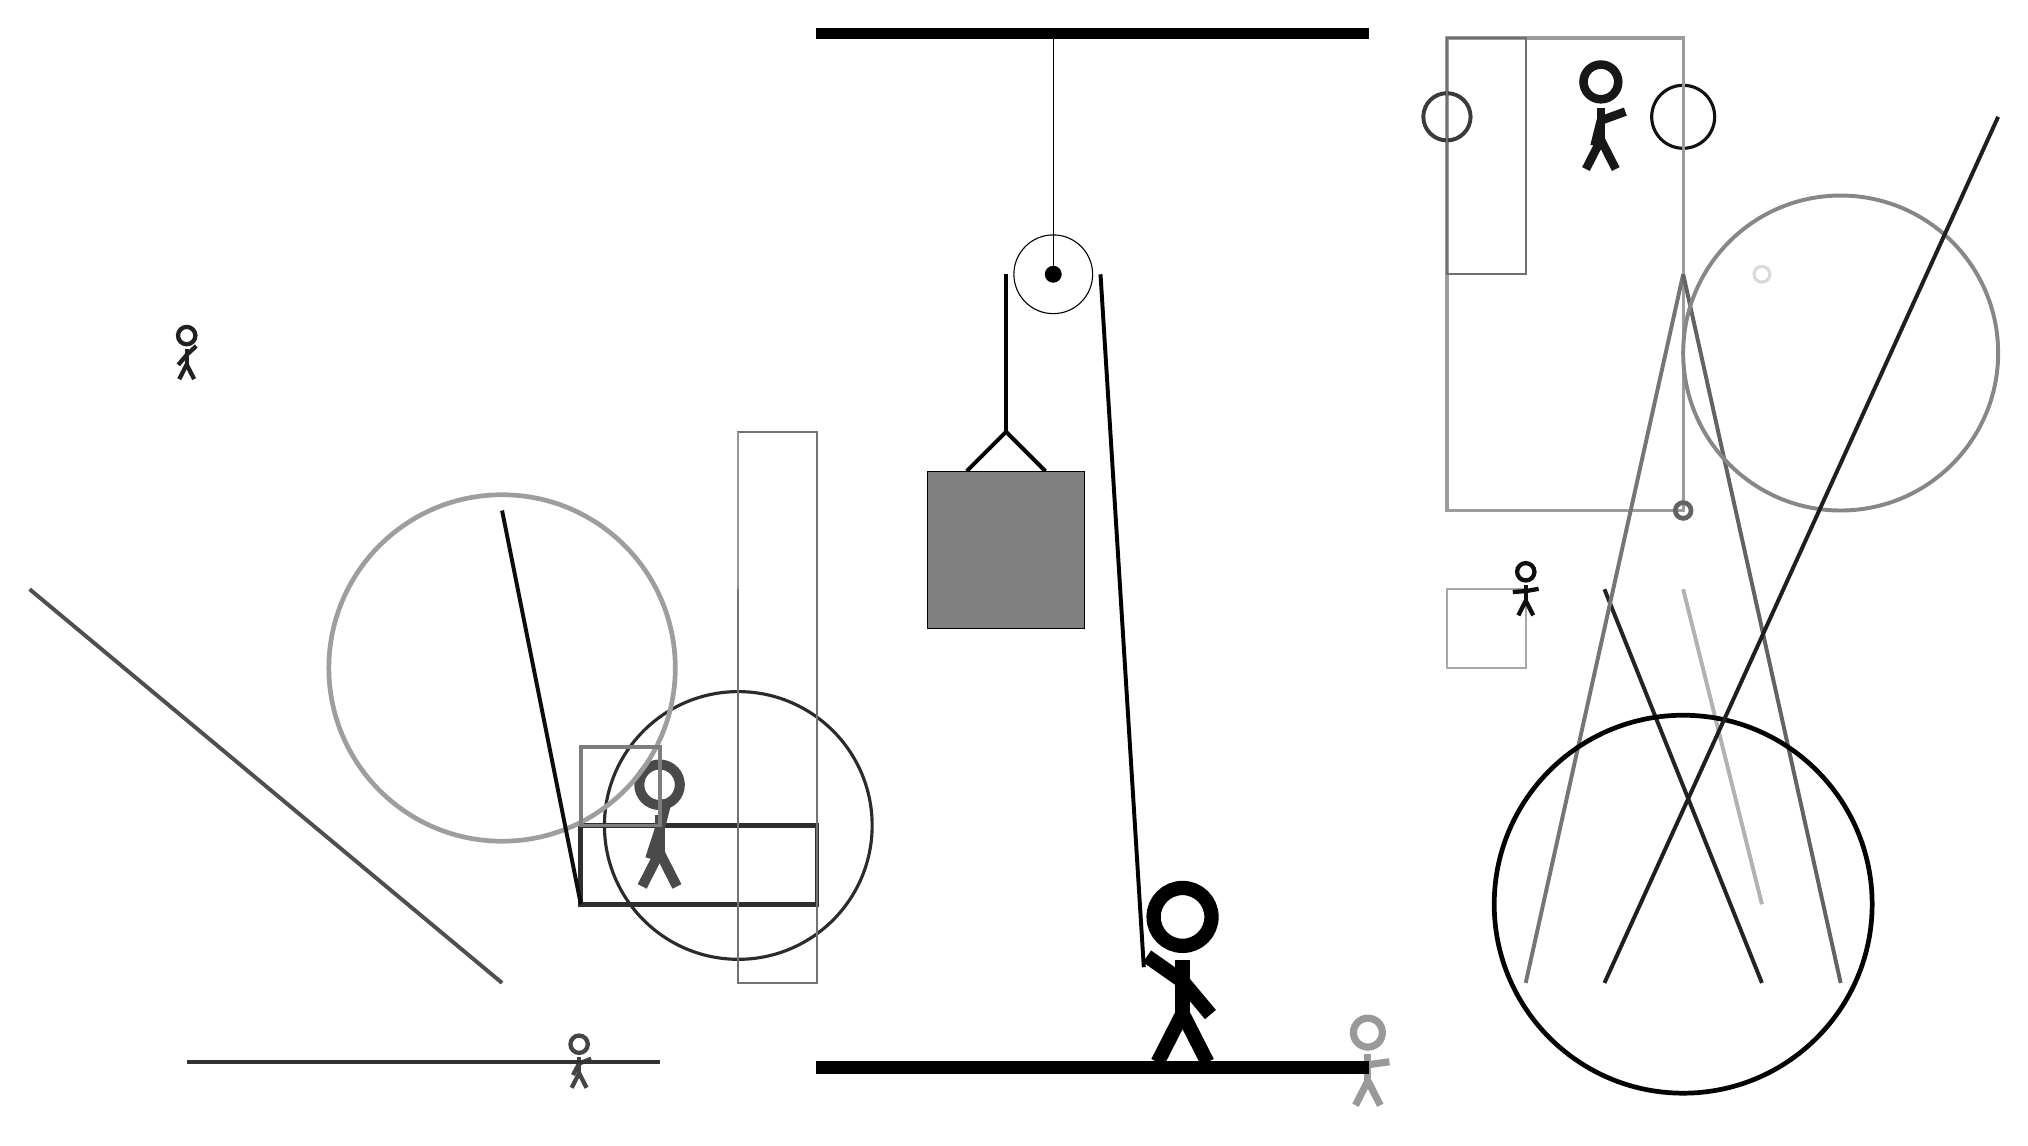
\begin{tikzpicture}
		%%%%% START %%%%%
		
		\draw[fill=black] (-2, 10) rectangle (5, 10.125);
		
		\draw[line width=0.5mm, color=black!86](8, 3) -- (10, -2);
		
		\draw[line width=0.6mm, color=black!82] (-2, 0) rectangle (-5, -1);
		\node[line width=0.3mm, color=black!73] at (-5, -3) {\Strichmaxerl[3][62][22]};
		\draw [line width=0.4mm, color=black!93](9, 9) circle (0.4);
		\node[line width=0.4mm, color=black!71] at (-4, 0) {\Strichmaxerl[7][72][76]};
		\draw [line width=0.4mm, color=black!83](-3, 0) circle (1.7);
		\draw[line width=0.3mm, color=black!55] (-2, -2) rectangle (-3, 5);
		\draw [line width=0.6mm, color=black!38](-6, 2) circle (2.2);
		\draw[line width=0.3mm, color=black!41] (-3, 3) rectangle (-3, 5);
		\draw[line width=0.3mm, color=black!34] (6, 3) rectangle (7, 2);
		\draw[line width=0.4mm, color=black!39] (6, 4) rectangle (9, 10);
		\node[line width=0.5mm, color=black!40] at (5, -3) {\Strichmaxerl[5][16][8]};
		\node[line width=0.2mm, color=black!91] at (8, 9) {\Strichmaxerl[6][76][20]};
		\draw[line width=0.5mm, color=black!30](10, -1) -- (9, 3);
		\draw[line width=0.5mm, color=black!80](-4, -3) -- (-10, -3);
		\draw[line width=0.5mm, color=black!69](-6, -2) -- (-12, 3);
		
		\draw[line width=0.5mm, color=black!54](7, -2) -- (9, 7);
		
		\draw[line width=0.5mm, color=black!61](9, 7) -- (11, -2);
		\node[line width=0.6mm, color=black!94] at (7, 3) {\Strichmaxerl[3][4][10]};
		
		\node[line width=0.3mm, color=black!87] at (-10, 6) {\Strichmaxerl[3][50][43]};
		\draw [line width=0.5mm, color=black!77](6, 9) circle (0.3);
		\draw [line width=0.6mm, color=black!99](9, -1) circle (2.4);
		\draw [line width=0.4mm, color=black!15](10, 7) circle (0.1);
		\draw [line width=0.5mm, color=black!47](11, 6) circle (2.0);
		\draw[line width=0.5mm, color=black!51] (-4, 0) rectangle (-5, 1);
		
		\draw[line width=0.5mm, color=black!88](8, -2) -- (13, 9);
		\draw[line width=0.2mm, color=black!56] (6, 10) rectangle (7, 7);
		\draw [line width=0.6mm, color=black!61](9, 4) circle (0.1);
		
		\draw[line width=0.5mm, color=black!95](-5, -1) -- (-6, 4);
		
		\draw (1, 7) circle (0.5);
		\draw[fill=black] (1, 7) circle (0.1);
		\draw (1, 10) -- (1, 7);
		
		\draw[line width=0.5mm] (-0.1, 4.5) -- (0.4, 5.0) -- (0.9, 4.5);
		\draw[fill=black!50] (-0.6, 4.5) rectangle (1.4, 2.5);
		
		\draw[line width=0.5mm] (0.4, 7) -- (0.4, 5.0);
		\centerarc[line width=0.5mm](1, 7)(0:180:0.6);
		\draw[line width=0.5mm](1.6, 7) -- (2.15, -1.8);
		
		\node at (2.6, -1.9) {\Strichmaxerl[10][-35][-50]};
		
		\draw[fill=black] (-2, -3) rectangle (5, -3.15);
		
		%%%%% END %%%%%
	\end{tikzpicture}
\end{document}